% ========================================
% Experimental Setups Section
% ========================================
\subsection{Experimental Setups}
We carried out our experiments on DAS-4 using OpenNebula platform. The
VM image we use is CentOS-5.4 whose image ID is 35, and our VM setup
is CPU=1, VCPU=2, with 1024MB memory.

We prepared three H.264 1080p movie trailers downloaded from Apple
Trailers\footnote{http://trailers.apple.com/trailers/}, which are
described in Table \ref{table_joblist}:

\begin{table}[!t]
  \caption{Jobs for Testings}
  \label{table_joblist}
  \centering
  \begin{tabular}{|l|l|l|l|}
    \hline
    Job Name & File Name & Encoding & File Size\\
    \hline
    \texttt{job1} & cloudatlas-trailer1b\_h1080p.mov & H.264 1080p & 172MB \\
    \hline
    \texttt{job2} & skyfall-tlr2\_h1080p.mov & H.264 1080p & 180MB \\
    \hline
    \texttt{job3} & taken2-tlr1\_h1080p.mov & H.264 1080p & 175MB \\
    \hline
  \end{tabular}
\end{table}

For testing the provisioning policies, we created three different jobs
with respect to these three files. Each job is to convert a H.264
1080p video file into an NTSC-DVD file. We then randomly generated
three workloads, each of which comprises of 40 jobs. The job arrival
times are generated using exponential distribution with three
different mean interval values: 10, 20, and 30 seconds.

\begin{table}[!t]
  \caption{Workloads for Testings}
  \label{table_workloadlist}
  \centering
  \begin{tabular}{|l|l|l|}
    \hline
    Workload Name & Number of Jobs & Job Arrival Time Distribution \\
    \hline
    \texttt{wl-10} & 40 & Exponential(10) \\
    \hline
    \texttt{wl-20} & 40 & Exponential(20) \\
    \hline
    \texttt{wl-30} & 40 & Exponential(30) \\
    \hline
  \end{tabular}
\end{table}


% ========================================
% Experiments
% ========================================
\subsection{Experiments}

% ========================================
% Benchmark Tests
% ========================================
\subsubsection{Benchmark Tests}
First, we did four benchmark tests to measure the performance of DAS-4
OpenNebula:

\begin{enumerate}
\item The first three tests run the three jobs separately. Each
  test is done 20 times, and we measure the job's running times
  (the total amount of time a job spent on its execution).
\item In another test, we continuously allocate and release a VM
  instance for 20 times in order to measure the overhead of allocating
  a VM instance on DAS-4.
\end{enumerate}

\begin{figure}[!t]
\centering
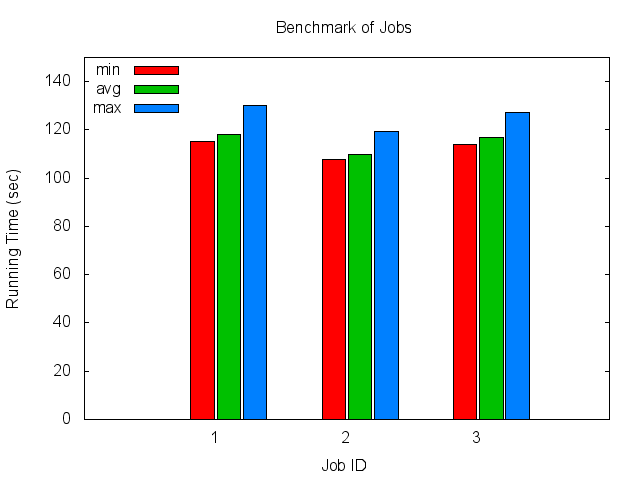
\includegraphics[width=0.35\textwidth]{pictures/benchmark-jobs.png}
\caption{Results of the benchmark tests for jobs}
\label{figure_jobbenchmark}
\end{figure}

As illustrated in Fig. \ref{figure_jobbenchmark}, all three jobs takes
almost the same amount of time to finish, with an average of 114.819 seconds, and there is no huge deviation from the average.

\begin{figure}
\centering

\includegraphics[width=0.35\textwidth]{pictures/vm-preparation-model.png}
\caption{VM Preparation Model}
\label{figure_vm_preparation_model}
\end{figure}

Figure \ref{figure_vm_preparation_model} is the model that we use to analyze
the VM allocation overhead. We measured the total preparation time of a VM,
which is the time from it is allocated until it is accessible through
\textsc{SSH}. The allocation time is from the VM instance is
allocated until its state becomes \staterunning, and the OS booting time is
the time after that and until this VM is accessible through \textsc{SSH}.

\begin{table}
\caption{Total Preparation Time of VMs}
\label{table_vm_preparation}
\centering
\begin{tabular}{|l|l|}
\hline
Average Total Preparation Time & 60.309 seconds \\
\hline
Average Allocation Time & $\approx$10 seconds \\
\hline
Average OS Booting Time & $\approx$50 seconds \\
\hline
\end{tabular}
\end{table}

Table \ref{table_vm_preparation} shows the results of our the VM allocation
overhead test. We only put the average values here because the minimum and
maximum values are close. The results suggest that the DAS-4 OpenNebula
is efficient in allocating a VM instance. It only takes approximately 10
seconds to become RUNNING after it is allocated. However, it takes
approximately 50 seconds for a VM to boot up its OS, which becomes the major
overhead of allocating a new VM.


% ========================================
% Experiments on the Provisioning Policies
% ========================================
\newcommand{\STATIC}{\textsc{static}}
\newcommand{\SE}{\textsc{se}}
\newcommand{\SEzero}{\textsc{se-0}}
\newcommand{\SEfive}{\textsc{se-5}}

\subsection{Experiments on the Provisioning Policies}
In this part, we use the three workloads to test the two policies. We
use three settings here:
\begin{enumerate}
\item \policystatic{} with 5 VMs. We call this \STATIC{} for short.
\item \policysimpleelastic{} that has 5 to 20 VMs, with \emph{threshold} set to 0. We call this \SEzero{} for short.
\item \policysimpleelastic{} that has 5 to 20 VMs, with \emph{threshold} set to 5. We call this \SEfive{} for short.
\end{enumerate}

\begin{figure}[!t]
\centering
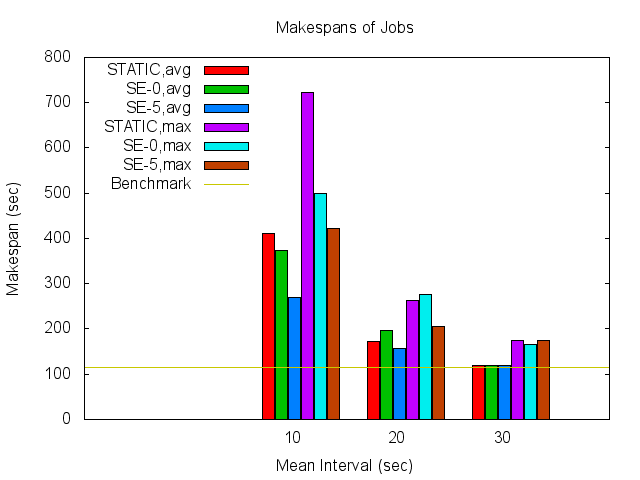
\includegraphics[width=0.35\textwidth]{pictures/all-makespans.png}
\caption{Makespans of jobs in the three workloads}
\label{figure_jobmakespan}
\end{figure}

Figure \ref{figure_jobmakespan} illustrates the job makespans of different
policies in each workload. The brown line indicates the average running time
of a job is the benchmark test. As expected, for \texttt{wl-10},
\SE{} outperforms the \STATIC{} both in the average case
and the worst case. \SEfive{} achieves the best job makespan for both
\texttt{wl-10} and \texttt{wl-20}. For \texttt{wl-30}, the performances are
almost the same, which suggests that five VMs are enough for \texttt{wl-30}.

Another observation is that, for \texttt{wl-10} and \texttt{wl-20}, the
average job makespans are both higher than the benchmark result. In another
test which we allocated 30 VMs, we find that there are totally 8 nodes being
used, each of which has 4 VMs or so on it. Also, comparing the detailed
job execution results (not present here), we find that DAS-4 OpenNebula's
over-allocation has a great impact on the VM performance. Computation, I/O
and network performances can all be influenced.

\begin{figure}[!t]
\centering
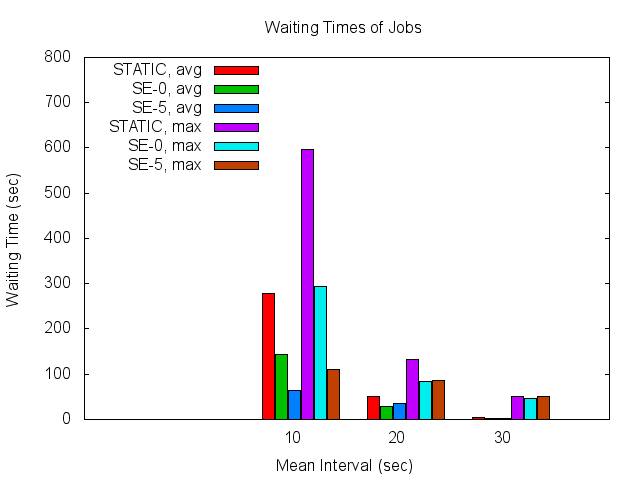
\includegraphics[width=0.35\textwidth]{pictures/all-waittimes.png}
\caption{Waiting times of jobs in the three workloads}
\label{figure_jobwaittime}
\end{figure}

For \texttt{wl-20}, Fig. \ref{figure_jobwaittime} shows that \SEzero{} has
the lowest job waiting time, however from \ref{figure_jobmakespan}, we
see that the job makespans are the highest. We believe that this slowdown
may be caused by DAS-4 OpenNebula's over-allocation of VMs. According to
our statistics, this slowdown can be 3.64 at max and 1.91 in average in
\textsc{wl-10}.

\begin{figure}[!t]
\centering
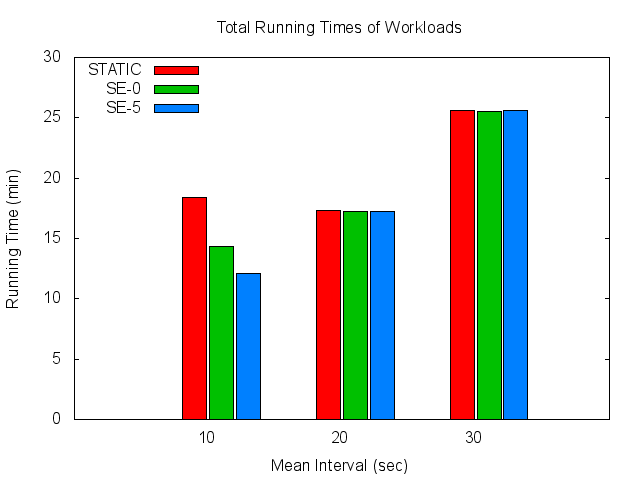
\includegraphics[width=0.35\textwidth]{pictures/workload-runtime.png}
\caption{Total makespan of three workloads}
\label{figure_workloadmakespan}
\end{figure}

The total makespans of each workload, which is depicted in Fig.
\ref{figure_workloadmakespan}, also suggests that \SE{}
achieves much better performance than \STATIC{} for \texttt{wl-10}.


% ========================================
% VM Performance Section
% ========================================
\subsection{VM Performances}\label{section_vm_performance}
We analyze the utilization of VMs in our system in this part. The
utilization level is the fraction of time VMs spent on running jobs
with respect to their total lifetime, and it can be described by
Equation \ref{equation_vm_util}.

\begin{equation}
\label{equation_vm_util}
Utilization = \frac{\sum{T_{running\_jobs}}}{\sum{T_{lifetime}}}
\end{equation}

\begin{figure}[!t]
\centering
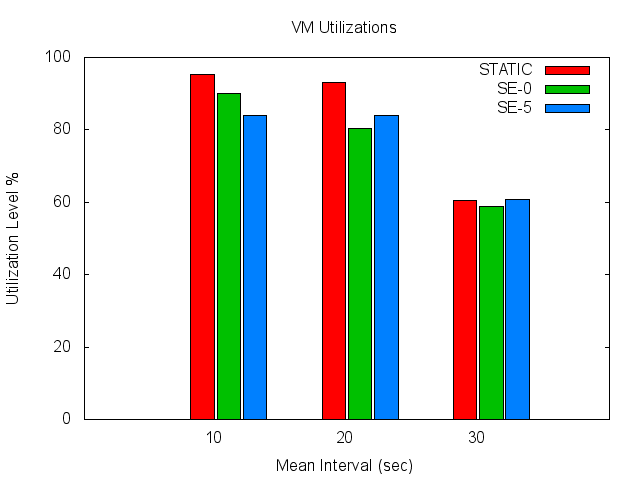
\includegraphics[width=0.35\textwidth]{pictures/vm-util.png}
\caption{VM Utilizations Levels}
\label{figure_vm_util}
\end{figure}

The results are illustrated in Fig. \ref{figure_vm_util}. Although in
\texttt{wl-10} and \texttt{wl-20}, the utilization levels of \SE{} are
lower than \STATIC{}, the decrements are acceptable. \SE{} can utilize
the VMs relatively efficiently.

Due to \SE{}'s feature that it terminates an idle VM as soon as there is
no pending jobs, we would also like to analyze its drawback.
For doing this, we measure the number of wasted VMs by using \SE{}.
A \emph{wasted VM} is a VM that has not got any job running on it during
its whole lifetime.

A VM can be wasted in this scenario: suppose we are using \SEzero{},
and there are 5 VMs in the system with 5 jobs running on them
respectively. Then a new job comes, and \SEzero{} will allocate a new VM,
say $VM_{new}$. However, before $VM_{new}$ becomes available, one
running job has been finished, which means a VM becomes idle, and this
new job is then assigned to this free VM. So, when $VM_{new}$ is
ready, the pending job queue is empty, and according to our policy,
$VM_{new}$ is terminated. In this case, no job has been running on
$VM_{new}$ during its lifetime, and we say that $VM_{new}$ is wasted.

In Fig. \ref{figure_vm_wasted}, we can see that in \texttt{wl-10},
the number of \SEzero is as high as 23, while \SEfive has no wasted VM
at all. \SEfive also has a low number of wasted VMs in the other two cases,
no exceeding 3.

\begin{figure}[!t]
\centering
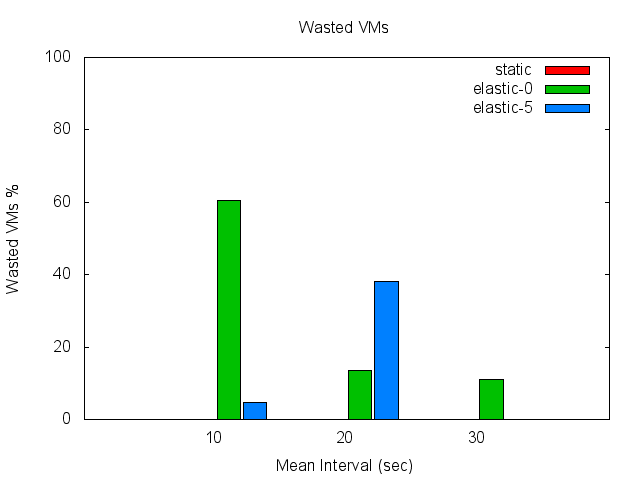
\includegraphics[width=0.35\textwidth]{pictures/vm-wasted.png}
\caption{Wasted VMs}
\label{figure_vm_wasted}
\end{figure}


% ========================================
% Speedup vs. Cost Tradeoff Section
% ========================================
\subsection{Speedup vs. Cost Tradeoff}
In this part, we calculate the speedups of using our SE provisioning
policy and the charged-costs. Because our VM setup has no
corresponding machine on Amazon Web Service, we use the charged cost
of m1.medium (\$0.16 per hour for Linux), which has two compute units,
for our charged-cost calculation. Table \ref{table_chargedcosts} shows
the results.

\begin{table}
\caption{Charged-costs}
\label{table_chargedcosts}
\centering
\begin{tabular}{|l|l|l|l|}
\hline
Workload & STATIC & SE-0 & SE-5 \\
\hline
\texttt{wl-10} & 1.54hrs (\$0.246) & 2.86hrs (\$0.458) & 2.73hrs (\$0.437) \\
\hline
\texttt{wl-20} & 1.44hrs (\$0.230) & 2.32hrs (\$0.371) & 1.62hrs (\$0.259) \\
\hline
\texttt{wl-30} & 2.13hrs (\$0.341) & 2.18hrs (\$0.349) & 2.13hrs (\$0.341) \\
\hline
\end{tabular}
\end{table}

\begin{table}
\caption{Speedups and Costs for wl-10}
\label{table_speedupcost}
\centering
\begin{tabular}{c|c|c|c|c|}
\cline{2-5}
 & \multicolumn{2}{c|}{\texttt{wl-10}} & \multicolumn{2}{c|}{\texttt{wl-20}} \\
\cline{2-5}
 & \SEzero & \textbf{\SEfive} & \SEzero & \textbf{\SEfive} \\
\hline
\multicolumn{1}{|c|}{Speedup} & 1.28 & \textbf{1.52} & 1.00 & \textbf{1.00} \\
\hline
\multicolumn{1}{|c|}{Cost} & 1.86 & \textbf{1.78} & 1.61 & \textbf{1.13} \\
\hline
\end{tabular}
\end{table}

We mainly focus on the results of \texttt{wl-10}, because this is the
only case that \SE outperforms \STATIC. From Table
\ref{table_speedupcost}, we can see that only \SEfive is close to
cost-speed proportional in both \texttt{wl-10} and \texttt{wl-20}.
The results suggest that it is not an easy task to achieve
cost-efficiency even in a simple cloud system.
